\chapter{Resultados}
\label{chap:resultados}

Este capítulo apresenta os resultados obtidos com a implementação do sistema
proposto. A avaliação foi dividida em duas etapas principais: uma análise
quantitativa, baseada em métricas automatizadas suportadas por \gls{LLM}s
(\textit{LLM-as-a-Judge}), e uma análise qualitativa, que examina a coerência
semântica e visual dos ativos gerados em cenários de teste específicos.

\section{Configuração Experimental}
\label{sec:configuracao_experimental}

Para validar a viabilidade e a eficácia do gerador de mapas, foram definidos
parâmetros fixos para a geração dos dos assets. Essa padronização é essencial
para garantir uma comparação justa entre os diferentes modelos de linguagem
avaliados.

O gerador foi configurado para produzir um número médio de elementos, buscando
um equilíbrio entre a diversidade de conteúdo e o tempo de processamento,
evitando a escassez de elementos, o que tornaria o jogo trivial, e o excesso de
informações, que poderia exceder a janela de contexto dos modelos menores. Os
parâmetros definidos para cada execução foram:

\begin{itemize}
    \item \textbf{Níveis da Masmorra:} 6 níveis de profundidade.
    \item \textbf{Inimigos:} 20 variações de inimigos.
    \item \textbf{Armas:} 30 tipos de armas.
\end{itemize}

\subsection{Modelos e Cenários de Teste}

Foram selecionados três \gls{LLM}s para a tarefa de geração, ordenados de forma
decrescente em relação à quantidade total de parâmetros, visando comparar
modelos robustos contra modelos otimizados para hardware com recursos limitados:

\begin{enumerate}
    \item \textbf{meta-llama/llama-4-maverick-17b-128e-instruct:} Modelo de
          maior escala baseado em arquitetura \gls{MOE}, contendo 400B de parâmetros
          totais (com 17B de parâmetros ativos durante a inferência), focado em alta
          aderência a instruções.
    \item \textbf{openai/gpt-oss-120b:} Modelo denso de grande porte (117B parâmetros,
          5.1B ativos), utilizado como referência de alta capacidade.
    \item \textbf{openai/gpt-oss-20b:} Modelo compacto (21B parâmetros, 3.6B ativos),
          projetado para eficiência, sendo o candidato ideal para validação de
          inferência em hardware local.
\end{enumerate}

Para a etapa de avaliação (\textit{LLM-based Evaluation}), utilizou-se o modelo
\textbf{Gemini 3 Pro} da Google como "juiz", devido à sua alta capacidade de
raciocínio e janela de contexto estendida. Para a métrica de reconstrução
semântica, empregou-se o modelo de \textit{embeddings}
\texttt{text-embedding-004}. Todos os modelos foram configurados com temperatura
de 0.4, um valor que balanceia criatividade e aderência às instruções, além de
ser um padrão em trabalhos atuais na área como o de
\citeauthor{nasir2024word2world}. Os testes foram conduzidos sobre cinco
\textit{prompts} (P1 a P5) abrangendo temas distintos, comuns ao gênero
\textit{roguelike}:

\begin{itemize}
    \item \textbf{P1:} \textit{The Cursed Dwarven Forge} (Medieval/Fantasia).
    \item \textbf{P2:} \textit{The Derelict Starship} (Ficção Científica/Espaço).
    \item \textbf{P3:} \textit{The Smuggler's Grotto} (Pirata/Náutico).
    \item \textbf{P4:} \textit{Neon Skyline Penthouse} (Cyberpunk/Urbano).
    \item \textbf{P5:} \textit{The Living Hive} (Alien/Bio-Horror).
\end{itemize}

\section{Análise Quantitativa}
\label{sec:analise_quantitativa}

A avaliação quantitativa focou em dois aspectos principais: a coerência do conteúdo gerado
e a fidelidade semântica (reconstrução).

A Tabela~\ref{tab:coerencia} apresenta os resultados da métrica de Coerência
(escala 0-100), avaliada pelo Gemini 3 Pro. Observa-se que o modelo
\texttt{gpt-oss-120b} obteve o melhor desempenho médio (93,6). O modelo
\texttt{llama-4-maverick-17b}, apesar de sua arquitetura massiva (400B),
apresentou uma média de 89 pontos. Importante notar o desempenho do modelo
compacto \texttt{gpt-oss-20b}, que atingiu média de 87,8 pontos. A proximidade
dos resultados do modelo menor em relação aos gigantes valida a hipótese de que
modelos compactos são viáveis para a geração procedural local, mantendo um nível
aceitável de coerência.

\begin{table}[h!]
    \centering
    \Caption{\label{tab:coerencia} Resultados da Métrica de Coerência (0-100)}
    \UFCtab{}{
        \begin{tabular}{lcccccc}
            \toprule
            \textbf{Modelo}      & \textbf{P1} & \textbf{P2} & \textbf{P3} & \textbf{P4} & \textbf{P5} & \textbf{Média} \\
            \midrule
            llama-4-maverick-17b & 95          & 65          & 92          & 95          & 98          & 89,0           \\
            openai/gpt-oss-120b  & 82          & 95          & 98          & 95          & 98          & \textbf{93,6}  \\
            openai/gpt-oss-20b   & 95          & 68          & 95          & 85          & 96          & 87,8           \\
            \bottomrule
        \end{tabular}
    }{
        \Fonte{Elaborado pelo autor}
    }
\end{table}

A Tabela~\ref{tab:reconstrucao} exibe a Métrica de Reconstrução Semântica
(Similaridade de Cosseno), que mede o quão bem os ativos gerados representam o
tema original. Todos os modelos apresentaram alta fidelidade, com valores médios
próximos a 0,89. O \texttt{gpt-oss-120b} obteve o melhor resultado individual no
P2 (0,921), indicando uma excelente capacidade de capturar as nuances do tema de
ficção científica, enquanto o modelo compacto \texttt{gpt-oss-20b} demonstrou
ser altamente competitivo, com média de 0,888.

\begin{table}[h!]
    \centering
    \Caption{\label{tab:reconstrucao} Resultados da Métrica de Reconstrução (Similaridade de Cosseno)}
    \UFCtab{}{
        \begin{tabular}{lcccccc}
            \toprule
            \textbf{Modelo}      & \textbf{P1} & \textbf{P2} & \textbf{P3} & \textbf{P4} & \textbf{P5} & \textbf{Média} \\
            \midrule
            llama-4-maverick-17b & 0,880       & 0,883       & 0,890       & 0,882       & 0,905       & 0,888          \\
            openai/gpt-oss-120b  & 0,877       & 0,921       & 0,908       & 0,895       & 0,867       & \textbf{0,894} \\
            openai/gpt-oss-20b   & 0,882       & 0,913       & 0,865       & 0,888       & 0,895       & 0,888          \\
            \bottomrule
        \end{tabular}
    }{
        \Fonte{Elaborado pelo autor}
    }
\end{table}

\section{Análise Qualitativa}
\label{sec:analise_qualitativa}

Para compreender a qualidade subjetiva e a coesão visual dos \textit{assets}
gerados, selecionaram-se dois casos de destaque para análise aprofundada: o
modelo \textbf{openai/gpt-oss-120b} no tema \textit{Sci-Fi} (P2), que obteve a
melhor reconstrução, e o modelo \textbf{meta-llama/llama-4-maverick-17b} no tema
\textit{Alien/Bio-Horror} (P5), que demonstrou alta especificidade em suas
instruções.

\subsection{Caso de Estudo 1: The Derelict Starship (GPT-120b)}

Neste cenário, o modelo gerou um pacote denominado "\textit{The Derelict - The
    Void-Strider Ark}". A descrição textual do ambiente evoca uma atmosfera de
horror industrial espacial, mencionando "painéis de aço reforçado", "dutos
expostos"\ e "vazamentos de vácuo".  A Figura~\ref{fig:p2_levels_player} ilustra
os níveis, o jogador e o objetivo final gerados. O jogador, "\textit{Void
    Strider}", é descrito como um sucateiro em um traje exoesqueleto. O sistema de
RAG recuperou corretamente um tile de personagem humanoide para representá-lo.
Os níveis progridem logicamente de "\textit{Hull Entryway}"\ (Entrada do Casco)
até "\textit{Command Bridge}"\ (Ponte de Comando), com texturas que refletem
ambientes metálicos e tecnológicos. O objetivo final, "\textit{Aurora Core
    Fragment}", está alinhado com a narrativa de uma IA corrompida.

\begin{figure}[!ht]
    \centering
    \Caption{\label{fig:p2_levels_player} Visualização dos níveis, jogador e objetivo final gerados (GPT-120b).}
    \UFCfig{}{
        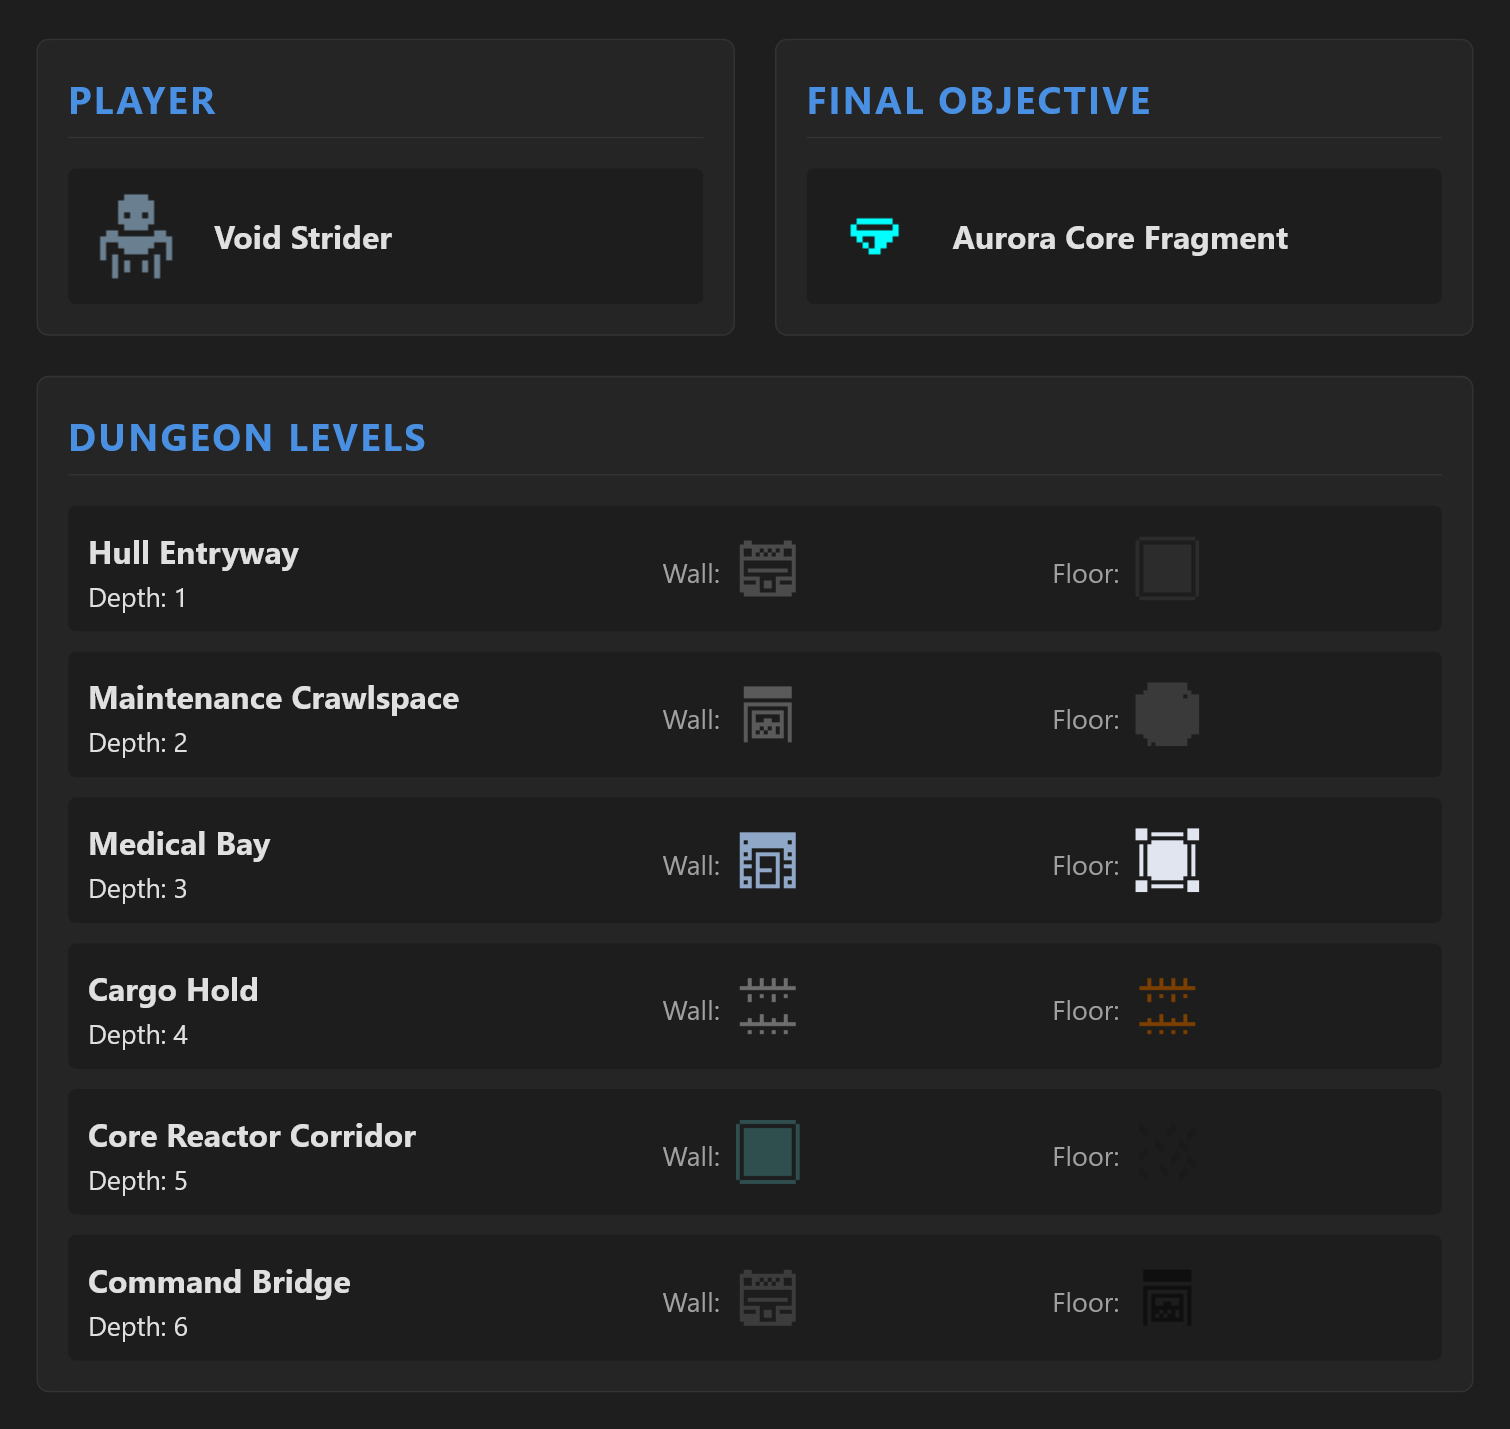
\includegraphics[width=8cm]{figuras/prompt2_gpt_120b_levels_player_and_final_objective.png}
    }{
        \Fonte{Elaborado pelo autor}
    }
\end{figure}

A coesão temática se estende aos inimigos (Figura \ref{fig:p2_enemies}) e armas
(Figura \ref{fig:p2_weapons}). Os inimigos incluem "\textit{Scout Spider}",
"\textit{Circuit Razor}"\ e o chefe "\textit{Core Sentinel}", todos descritos
como drones ou construtos mecânicos. As texturas recuperadas exibem tons de
cinza, azul e vermelho, típicos de máquinas. As armas, como "\textit{Plasma
    Pistol}"\ e "\textit{Arc Welder Sword}", misturam tecnologia futurista com
ferramentas industriais improvisadas, reforçando o tema de sobrevivência em uma
nave abandonada.

\begin{figure}[!ht]
    \centering
    \Caption{\label{fig:p2_weapons} Armas geradas (GPT-120b).}
    \UFCfig{}{
        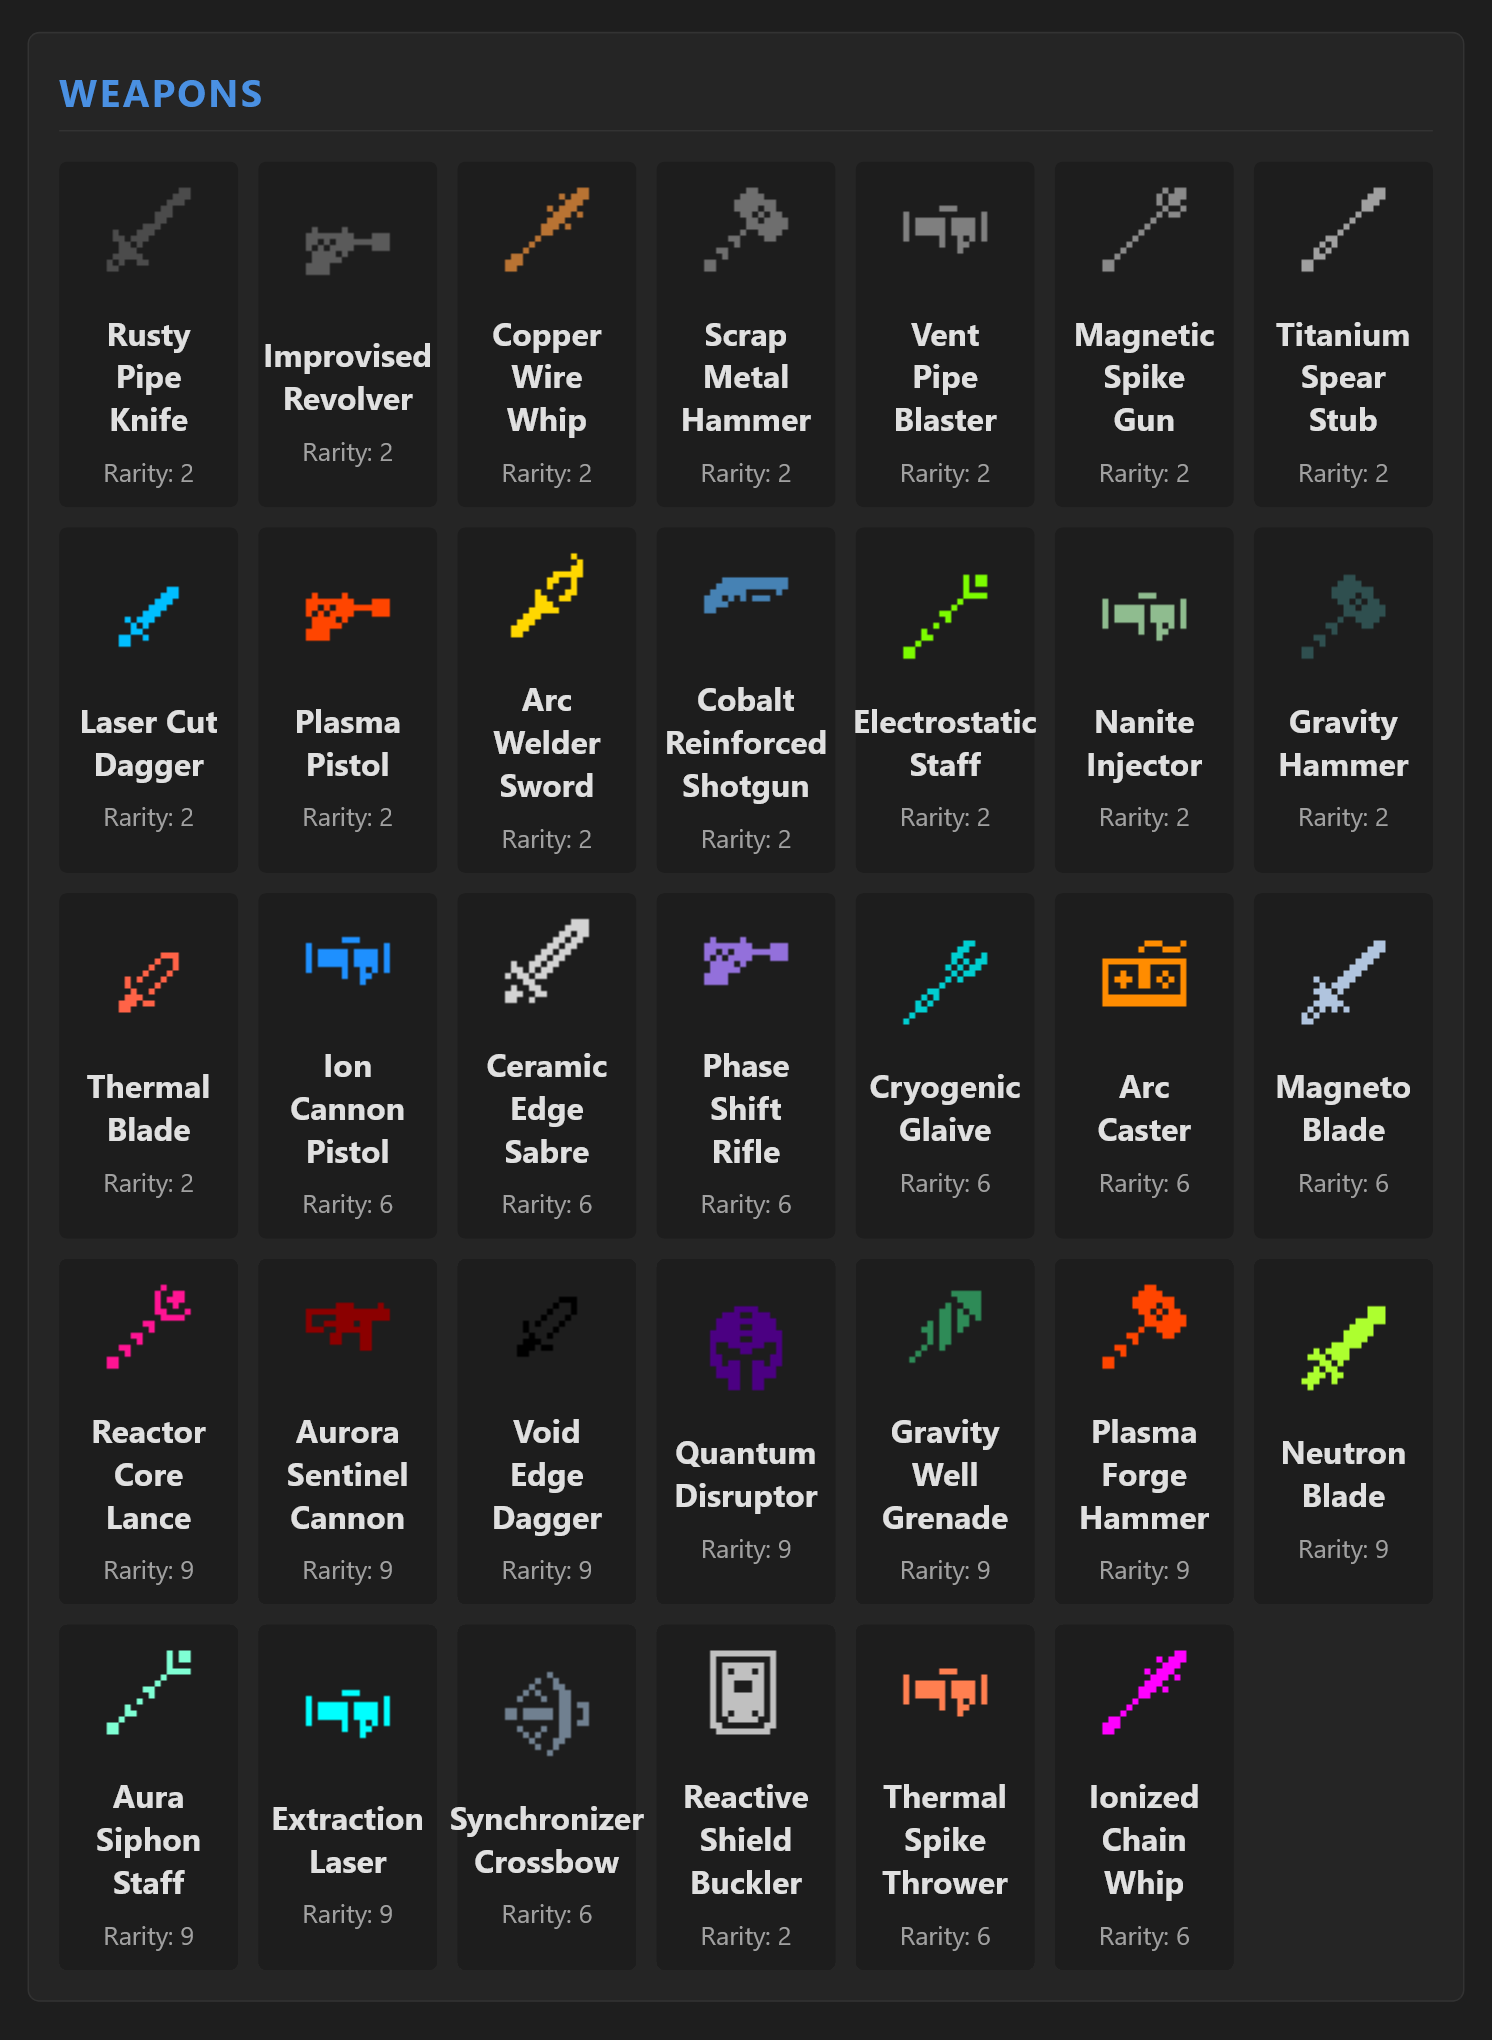
\includegraphics[width=8cm]{figuras/prompt2_gpt_120b_weapons.png}
    }{
        \Fonte{Elaborado pelo autor}
    }
\end{figure}

\begin{figure}[!ht]
    \centering
    \Caption{\label{fig:p2_enemies} Inimigos gerados (GPT-120b).}
    \UFCfig{}{
        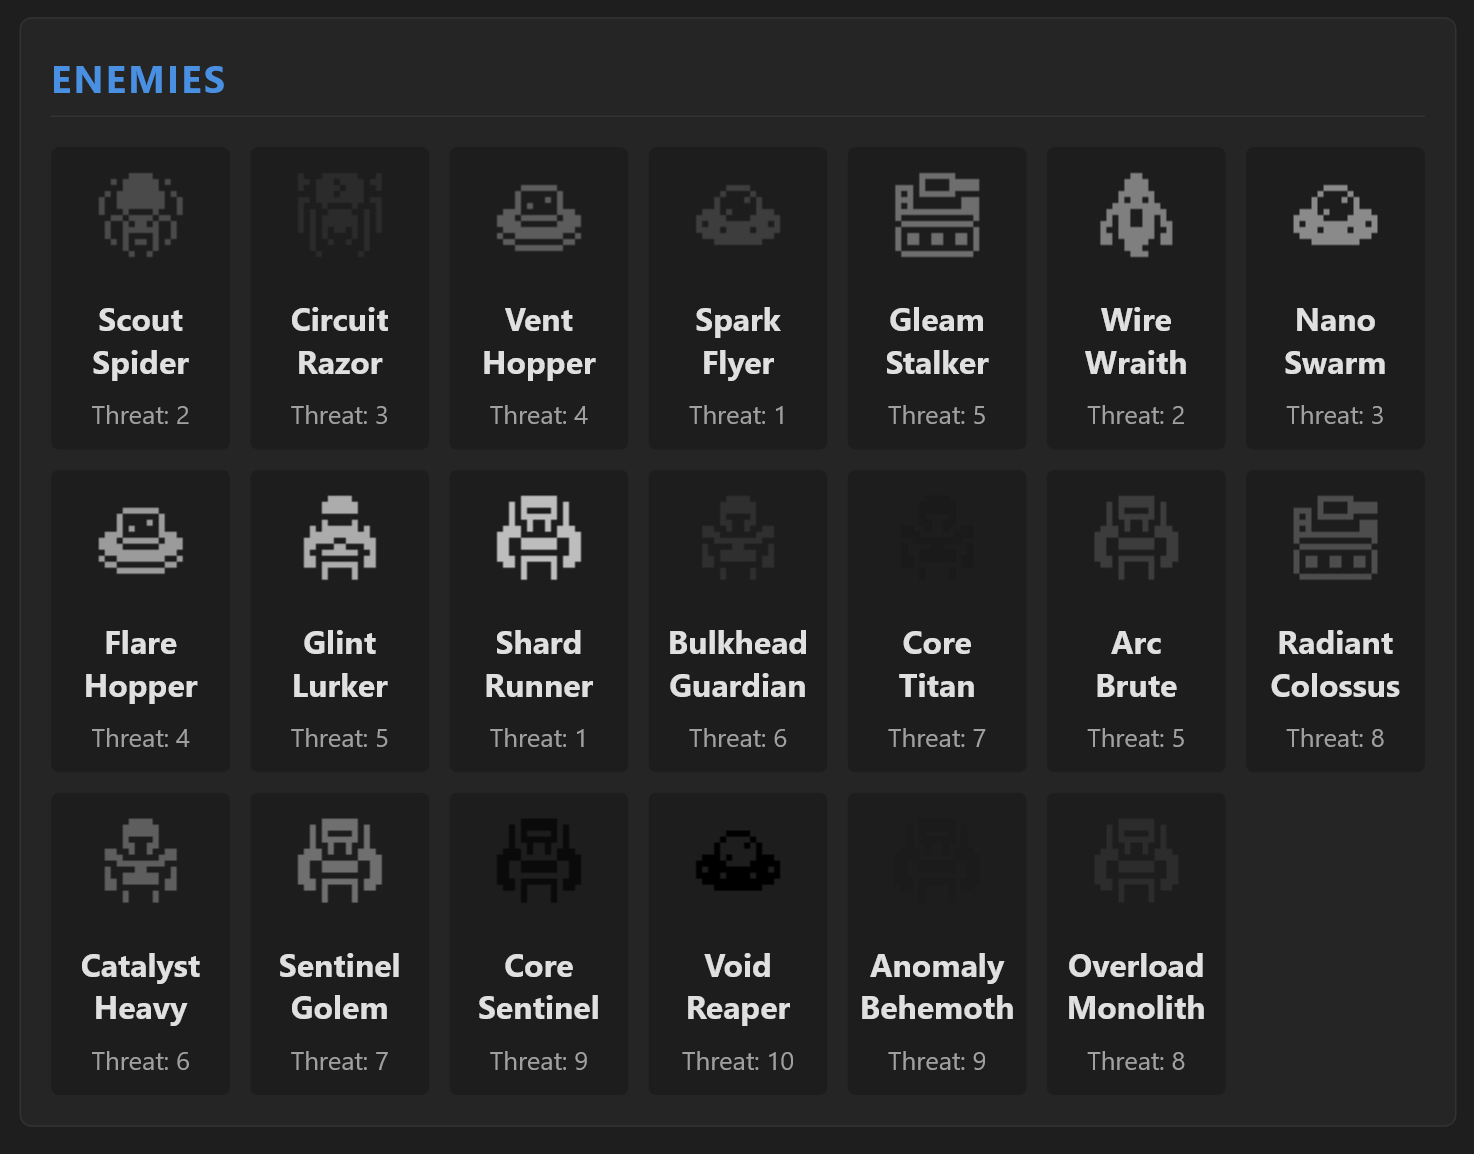
\includegraphics[width=8cm]{figuras/prompt2_gpt_120b_enemies.png}
    }{
        \Fonte{Elaborado pelo autor}
    }
\end{figure}

\subsection{Caso de Estudo 2: The Living Hive (Llama-17b)}

O modelo Llama-17b demonstrou excepcional capacidade de adaptação ao tema de
horror biológico no cenário P5, gerando o pacote "\textit{Gutrixa}". Tirando
proveito de sua vasta quantidade de parâmetros totais (400B) e treinamento em
instruções, o modelo construiu uma narrativa que descreve o interior de um
organismo colossal, rejeitando linhas retas em favor de "tecidos musculares" e
"câmaras esféricas".

A Figura~\ref{fig:p5_levels_player} apresenta os resultados estruturais. O
jogador é um "\textit{Twisted Cultist}"\ (Cultista Distorcido), cuja história de
fundo envolve uma seita que adora a criatura planetária. Os níveis, como
"\textit{The Caverns of Corruption}"\ e "\textit{The Heart of Corruption}",
utilizam texturas orgânicas e cores vibrantes (roxo, verde, rosa), contrastando
fortemente com o exemplo anterior.

\begin{figure}[!ht]
    \centering
    \Caption{\label{fig:p5_levels_player} Visualização dos níveis, jogador e objetivo final gerados (Llama-17b).}
    \UFCfig{}{
        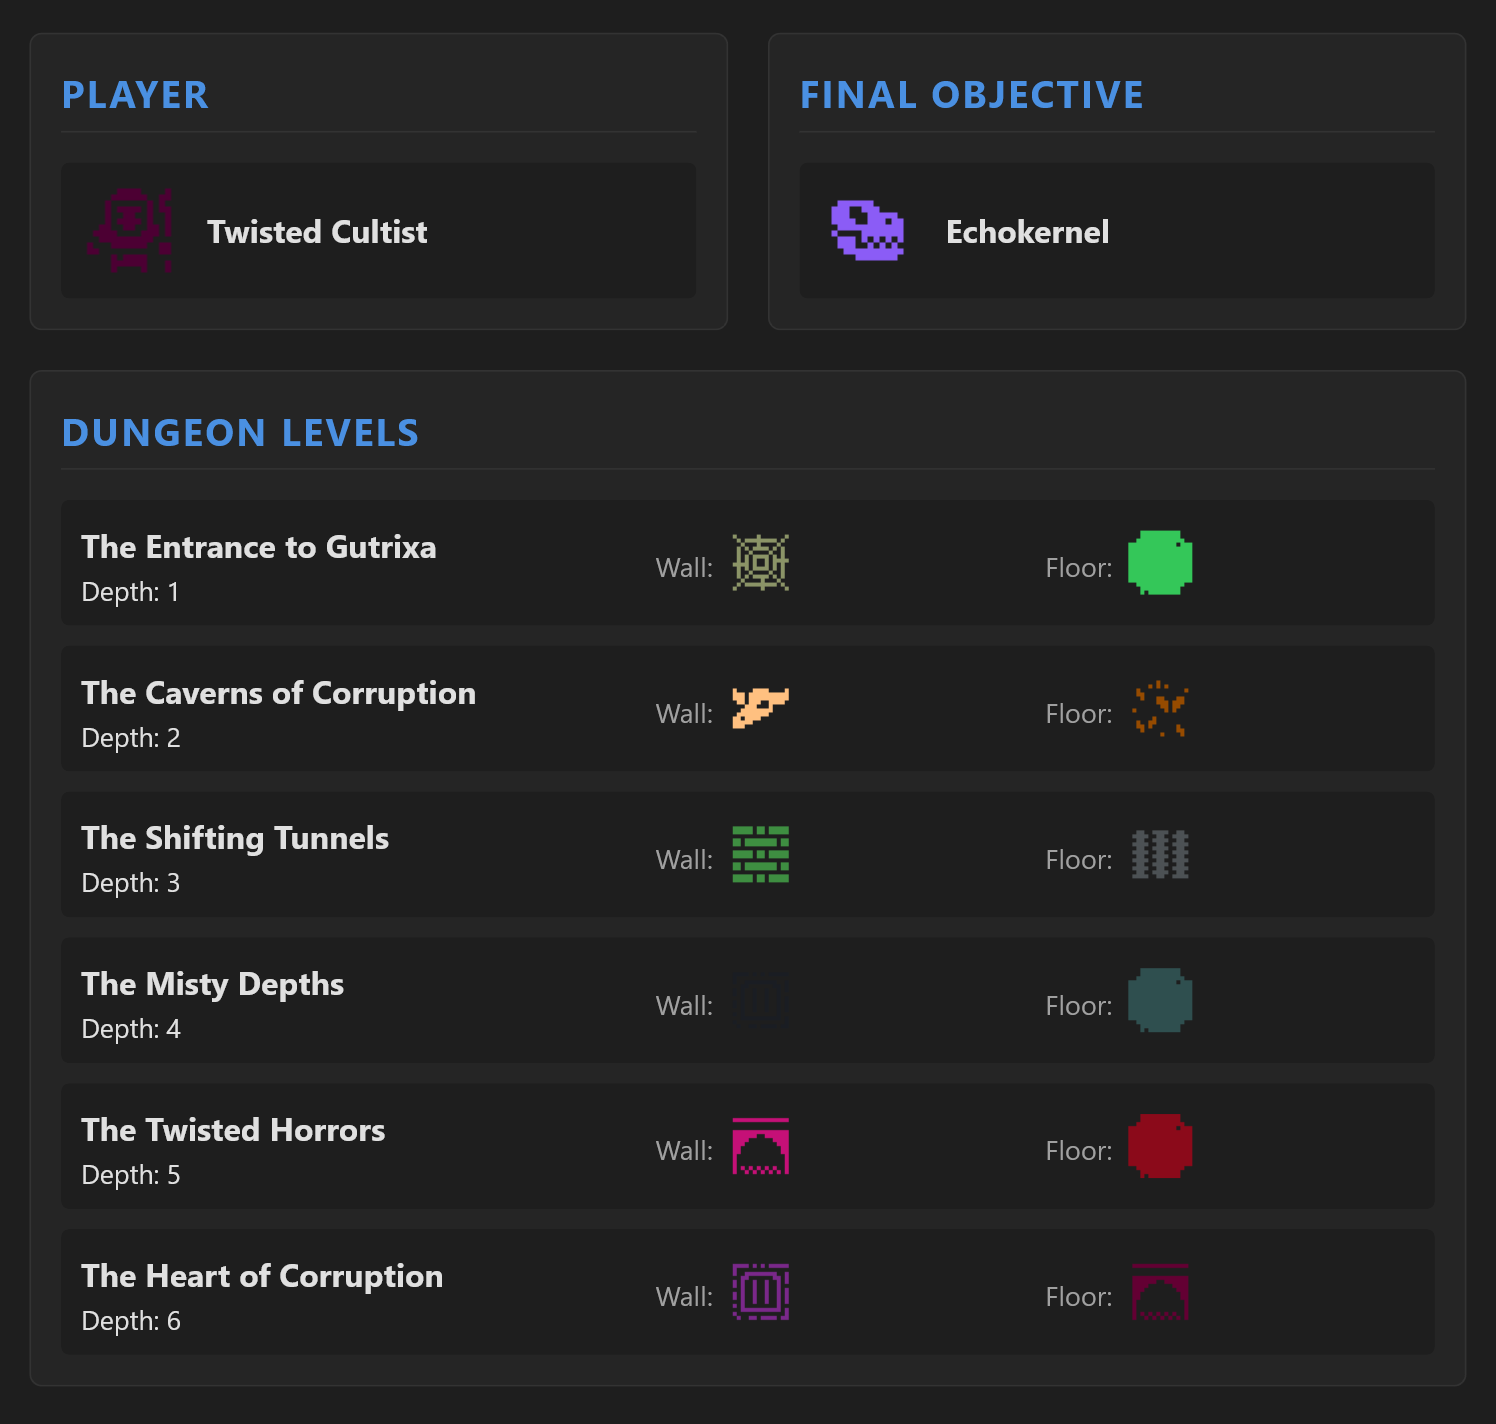
\includegraphics[width=8cm]{figuras/prompt5_llama_17b_levels_player_and_final_objective.png}
    }{
        \Fonte{Elaborado pelo autor}
    }
\end{figure}

Os inimigos gerados (Figura \ref{fig:p5_enemies}) reforçam o tema grotesco, com
criaturas como "\textit{Gutrixa Groaner}", "\textit{Flesh Borer}"\ e
"\textit{Zhathik Titan}". As descrições enfatizam características insectoides e
carnosas. As armas (Figura \ref{fig:p5_weapons}), como "\textit{Flesh Forged
Dagger}"\ e "\textit{Acid Sprayer}", utilizam materiais orgânicos (ossos,
tendões) em vez de metal, demonstrando que o modelo compreendeu a restrição de
materiais do mundo. O objetivo final, "\textit{Echokernel}", é descrito como o
coração corrompido da entidade, fechando o ciclo narrativo.

\begin{figure}[!ht]
    \centering
    \Caption{\label{fig:p5_weapons} Armas geradas (Llama-17b).}
    \UFCfig{}{
        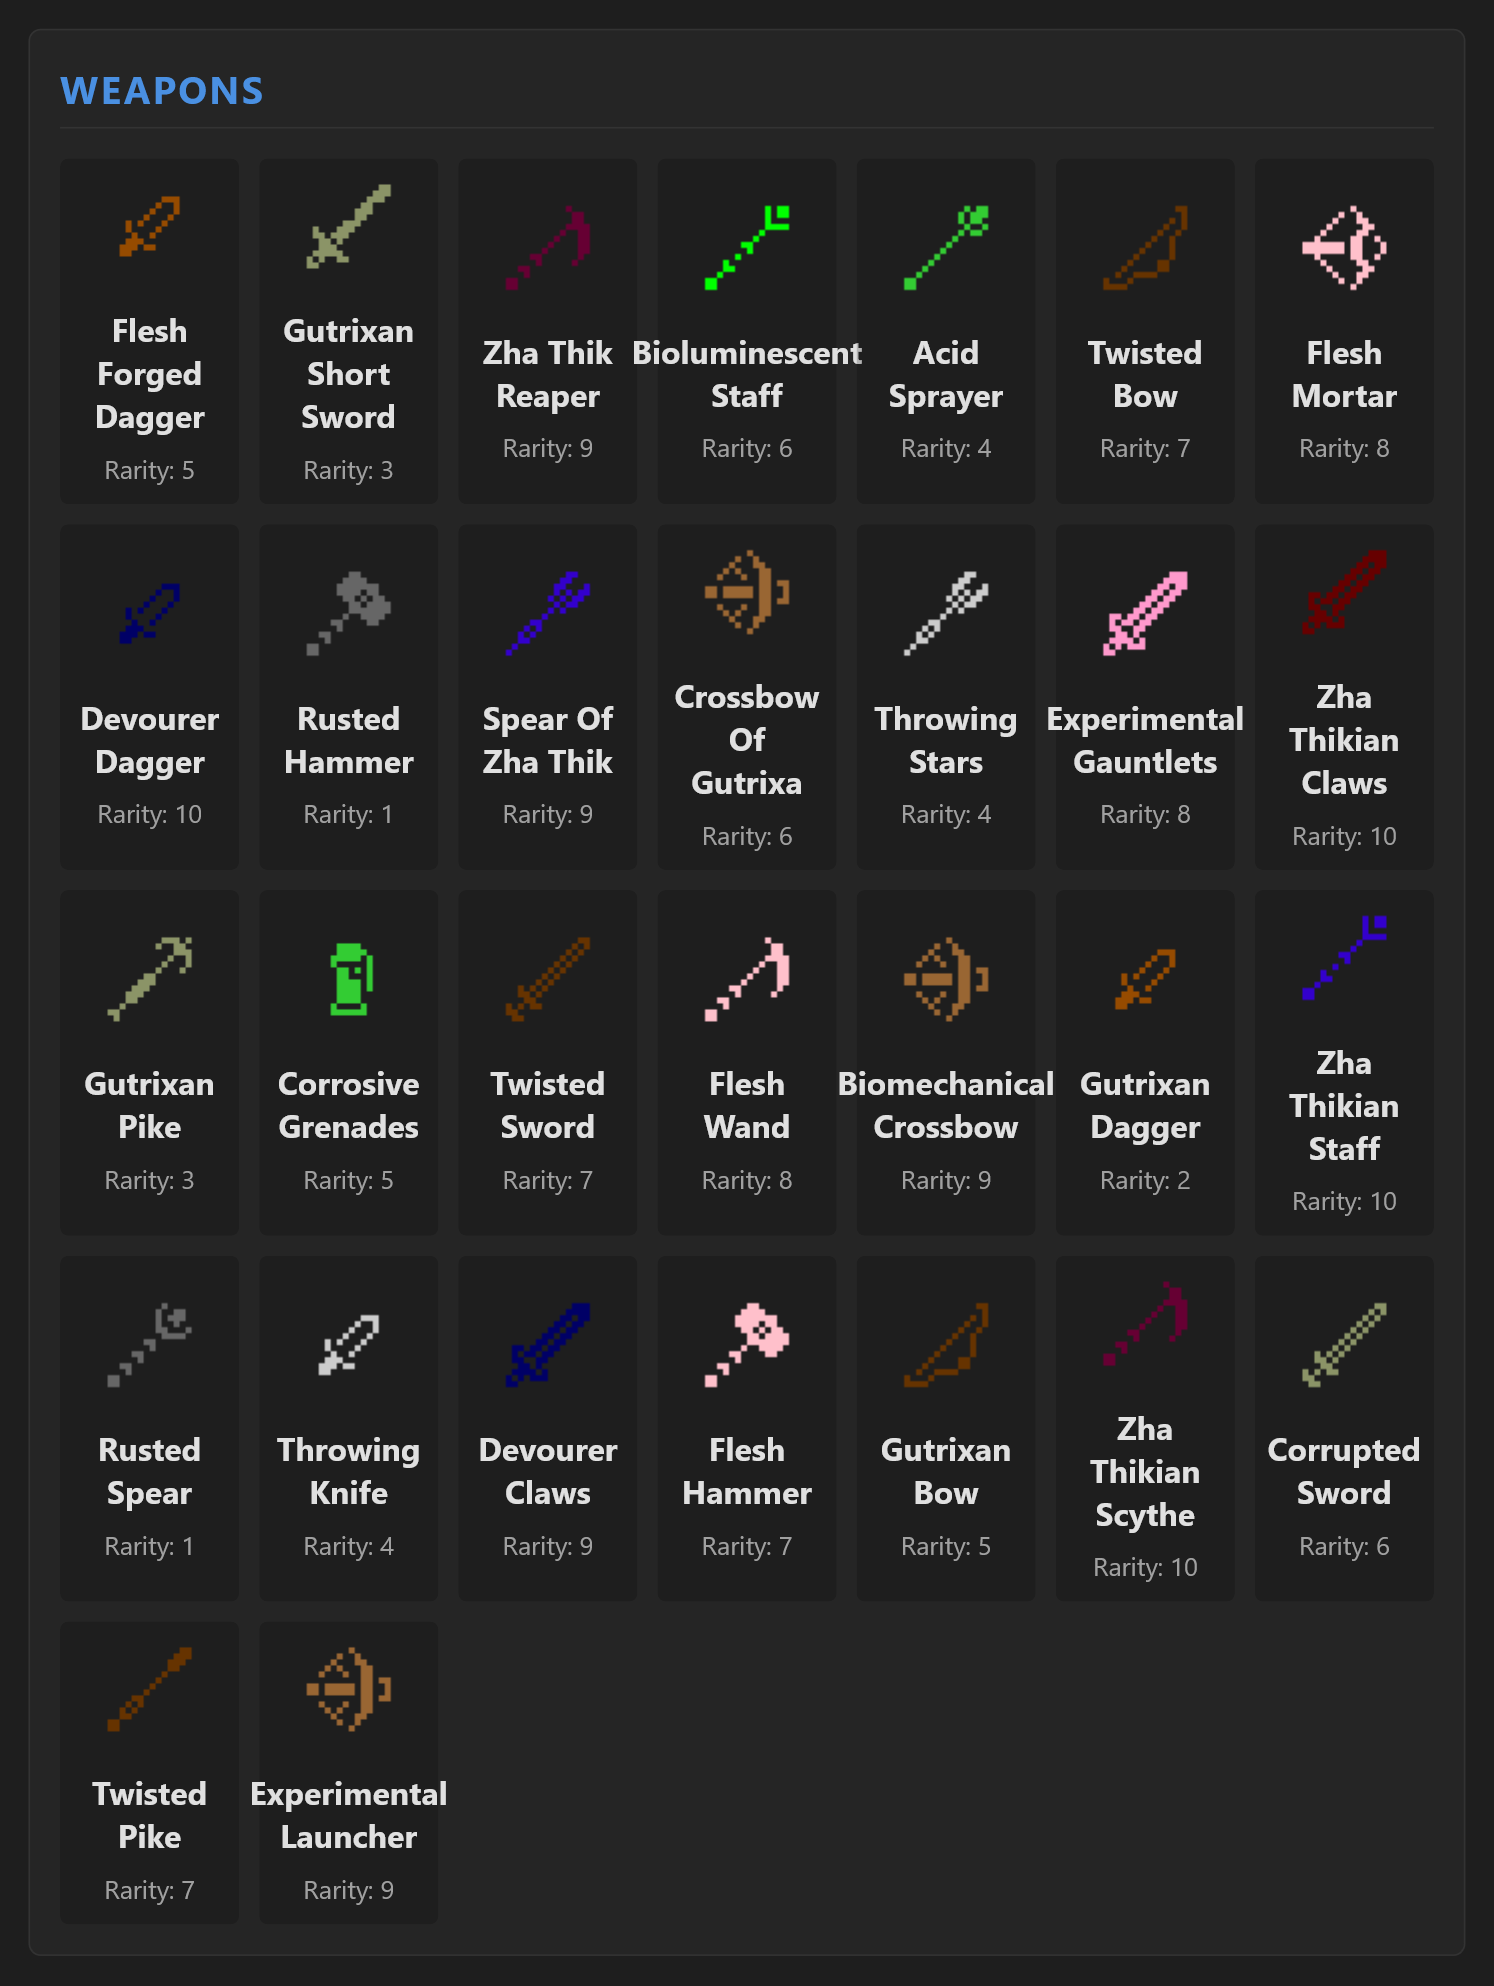
\includegraphics[width=8cm]{figuras/prompt5_llama_17b_weapons.png}
    }{
        \Fonte{Elaborado pelo autor}
    }
\end{figure}

\begin{figure}[!ht]
    \centering
    \Caption{\label{fig:p5_enemies} Inimigos gerados (Llama-17b).}
    \UFCfig{}{
        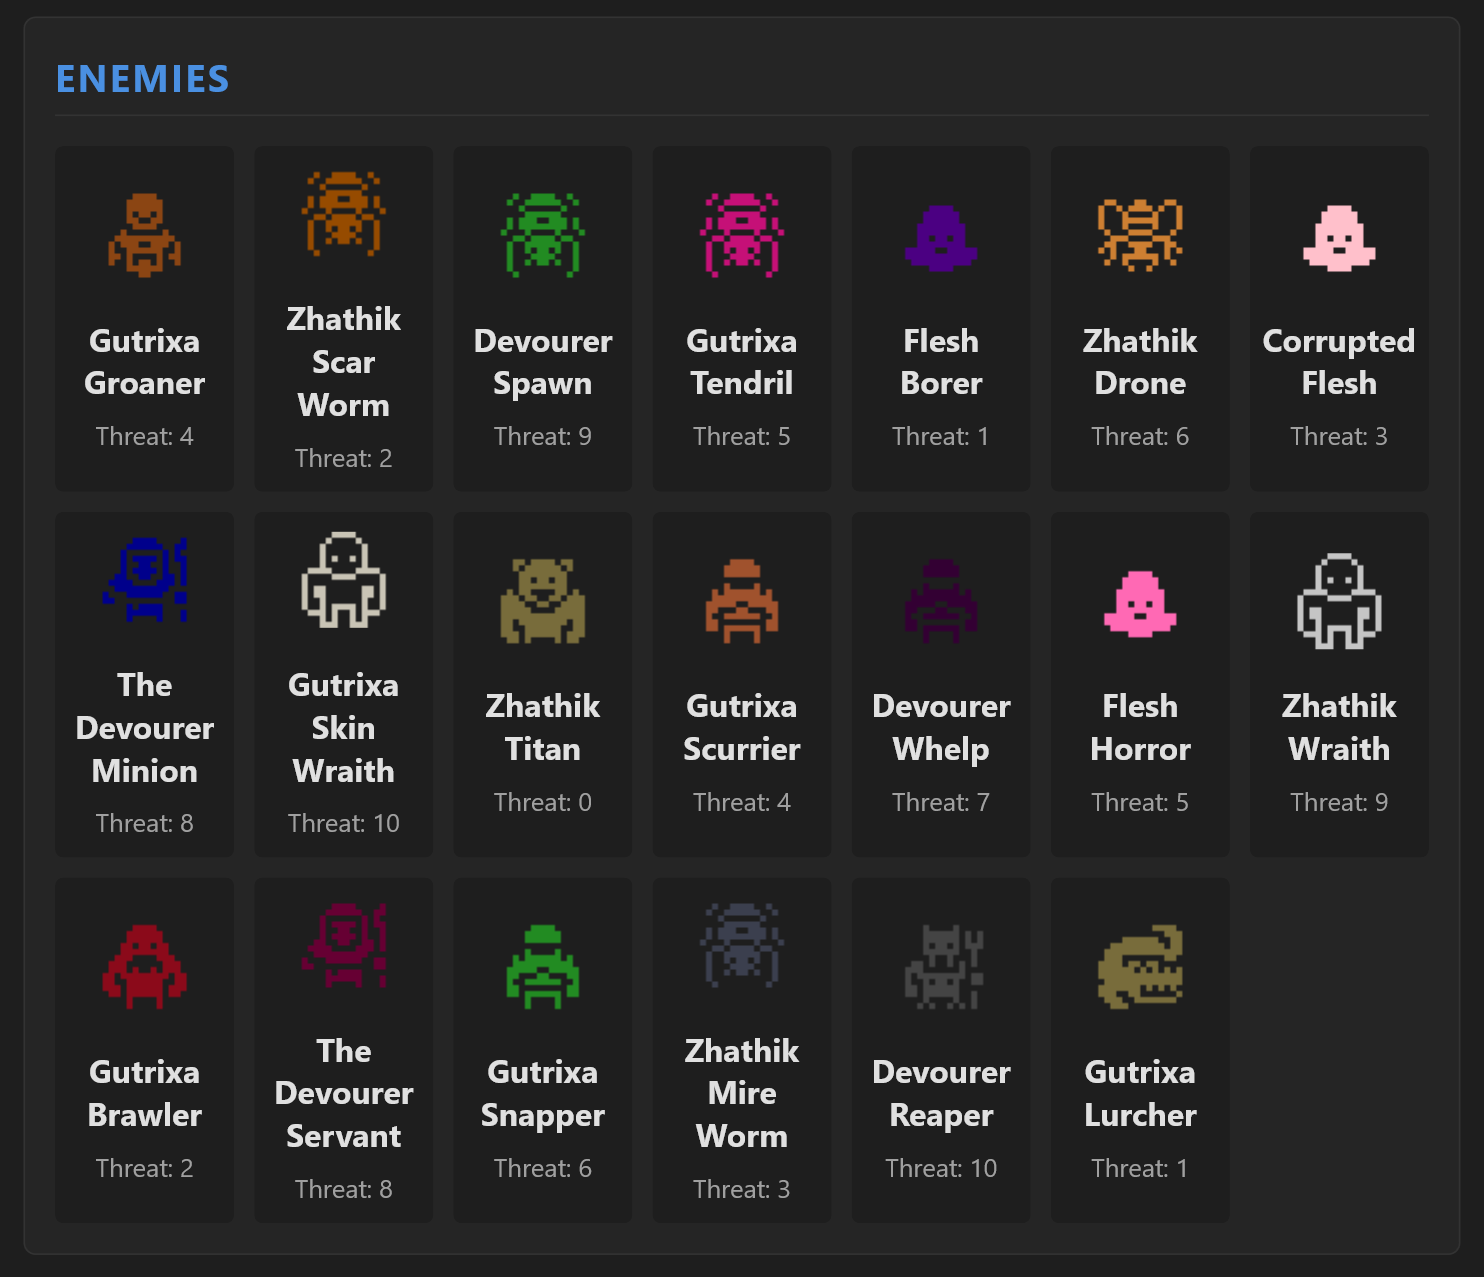
\includegraphics[width=8cm]{figuras/prompt5_llama_17b_enemies.png}
    }{
        \Fonte{Elaborado pelo autor}
    }
\end{figure}

A comparação qualitativa indica que, embora o GPT-120b tenda a gerar descrições
ligeiramente mais detalhadas, o modelo Llama-17b foi capaz de capturar a
essência estilística do tema com precisão surpreendente, selecionando paletas de
cores e terminologias adequadas (ex: "\textit{flesh}", "\textit{sinew}", "\textit{chitinous}") que guiaram
o sistema de \gls{RAG} para texturas visualmente distintas do cenário de ficção
científica.

\section{Jogo Roguelike}
\label{sec:implementacao_roguelike}

Além da geração dos ativos textuais e visuais, uma etapa fundamental deste
trabalho foi a validação destes elementos em um ambiente de jogo funcional.
Utilizando a \textit{game engine Godot} em sua versão 4.5.1, foi desenvolvido um
jogo \textit{Roguelike} capaz de processar um \textit{AssetBundle} em formato
\gls{JSON} e transformá-lo em um mapa jogável. Esta seção detalha os sistemas
básicos implementados que compõem a experiência de jogo, desde a interface do
usuário até os algoritmos de visibilidade e distribuição
procedural.

\subsection{Interface e Ciclo de Gameplay}

A Figura~\ref{fig:full_vision} apresenta uma visão geral da interface principal
do jogo durante uma partida. A implementação segue estritamente as convenções do
gênero. O núcleo do jogo opera através de um sistema de turnos, exibido no
canto esquerdo da tela (abaixo das barras de status). Os turnos são
incrementados apenas após o jogador realizar uma ação significativa, como
mover-se, atacar ou utilizar um item. Esta mecânica é crucial para o aspecto
tático do gênero, permitindo que o jogador tenha tempo ilimitado para planejar
suas ações, decidir entre atacar um inimigo próximo, utilizar uma poção de cura
ou recuar estrategicamente, antes que o ambiente reaja.

\begin{figure}[!ht]
    \centering
    \Caption{\label{fig:full_vision} Visão geral da interface do jogo,
        destacando HUD, logs e inventário.}
    \UFCfig{}{
        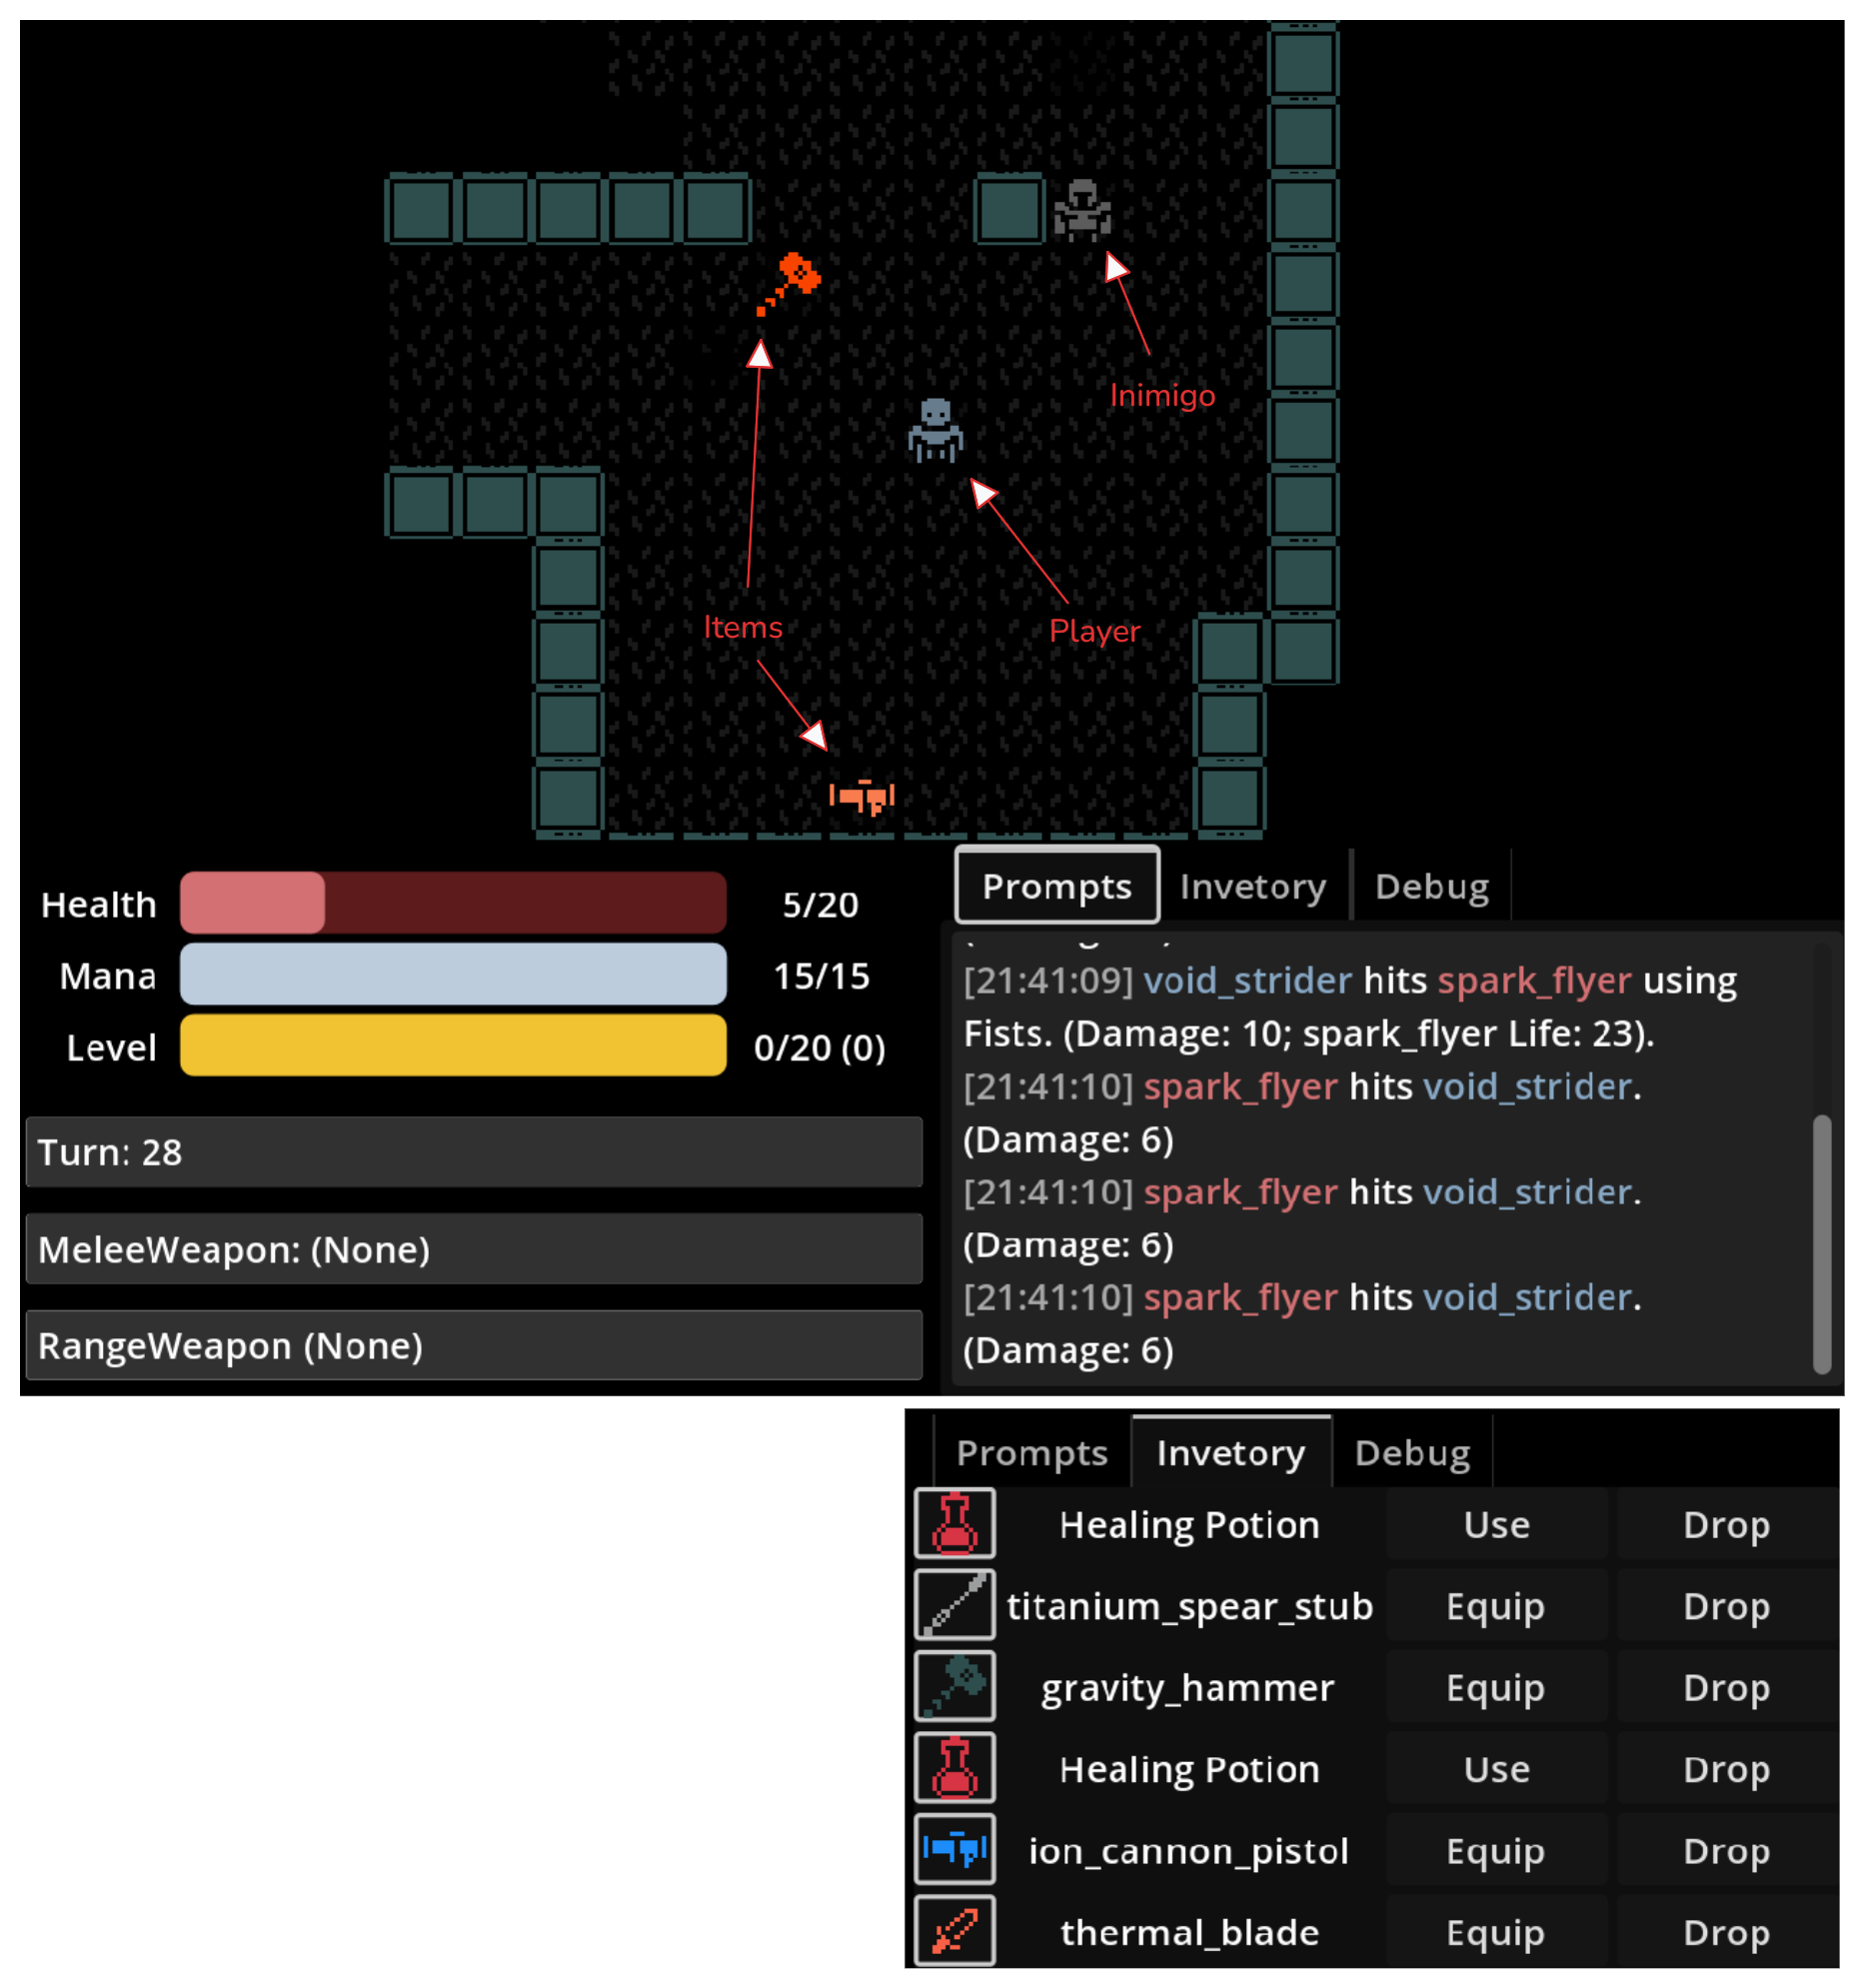
\includegraphics[width=12cm]{figuras/full_vizion_of_the_game.png}
    }{
        \Fonte{Elaborado pelo autor}
    }
\end{figure}

No canto inferior esquerdo, o \gls{HUD} fornece informações sobre o estado do
personagem através de três barras de progresso:
\begin{itemize}
    \item \textbf{Barra Vermelha (Vida):} Representa a saúde do jogador. Se esta
          barra chegar a zero, o personagem morre, resultando na perda de todos os
          itens e do progresso atual, forçando o reinício em um novo mapa gerado
          aleatoriamente.
    \item \textbf{Barra Azul (Mana):} Indica o recurso necessário para a
          utilização de armas de longo alcance.
    \item \textbf{Barra Amarela (Experiência):} Monitora o progresso do jogador.
          Ao atingir o máximo, o personagem sobe de nível, restaurando e incrementando
          seus atributos máximos de vida e mana.
\end{itemize}

Abaixo das barras, são exibidos os nomes da arma corpo a corpo (\textit{melee})
e da arma de ataque à distância atualmente equipadas. No lado direito da tela,
uma barra de menus permite ao jogador alternar entre duas abas principais:
\textit{"Prompts"} e \textit{"Inventory"}. A aba de \textit{Prompts} atua como
um registro de eventos (\textit{combat log}), exibindo mensagens informativas
como dano causado ou recebido e descrições de itens encontrados no chão. A aba
de \textit{Inventory} permite o gerenciamento de recursos. O jogador pode
equipar armas coletadas ou consumir itens como poções de cura e mana. A cena é
composta ainda pela renderização do mapa, no qual é possível observar o jogador
centralizado, itens espalhados pelo chão e inimigos patrulhando a área.

\subsection{Sistema de Campo de Visão (FOV)}

A exploração e a descoberta são pilares dos \textit{roguelikes}. Para suportar
isso, foi implementado um sistema de Campo de Visão , ilustrado na Figura~\ref{fig:fov}.

\begin{figure}[!ht]
    \centering
    \Caption{\label{fig:fov} Sistema de Campo de Visão: distinção entre áreas
        visíveis, exploradas e não exploradas.}
    \UFCfig{}{
        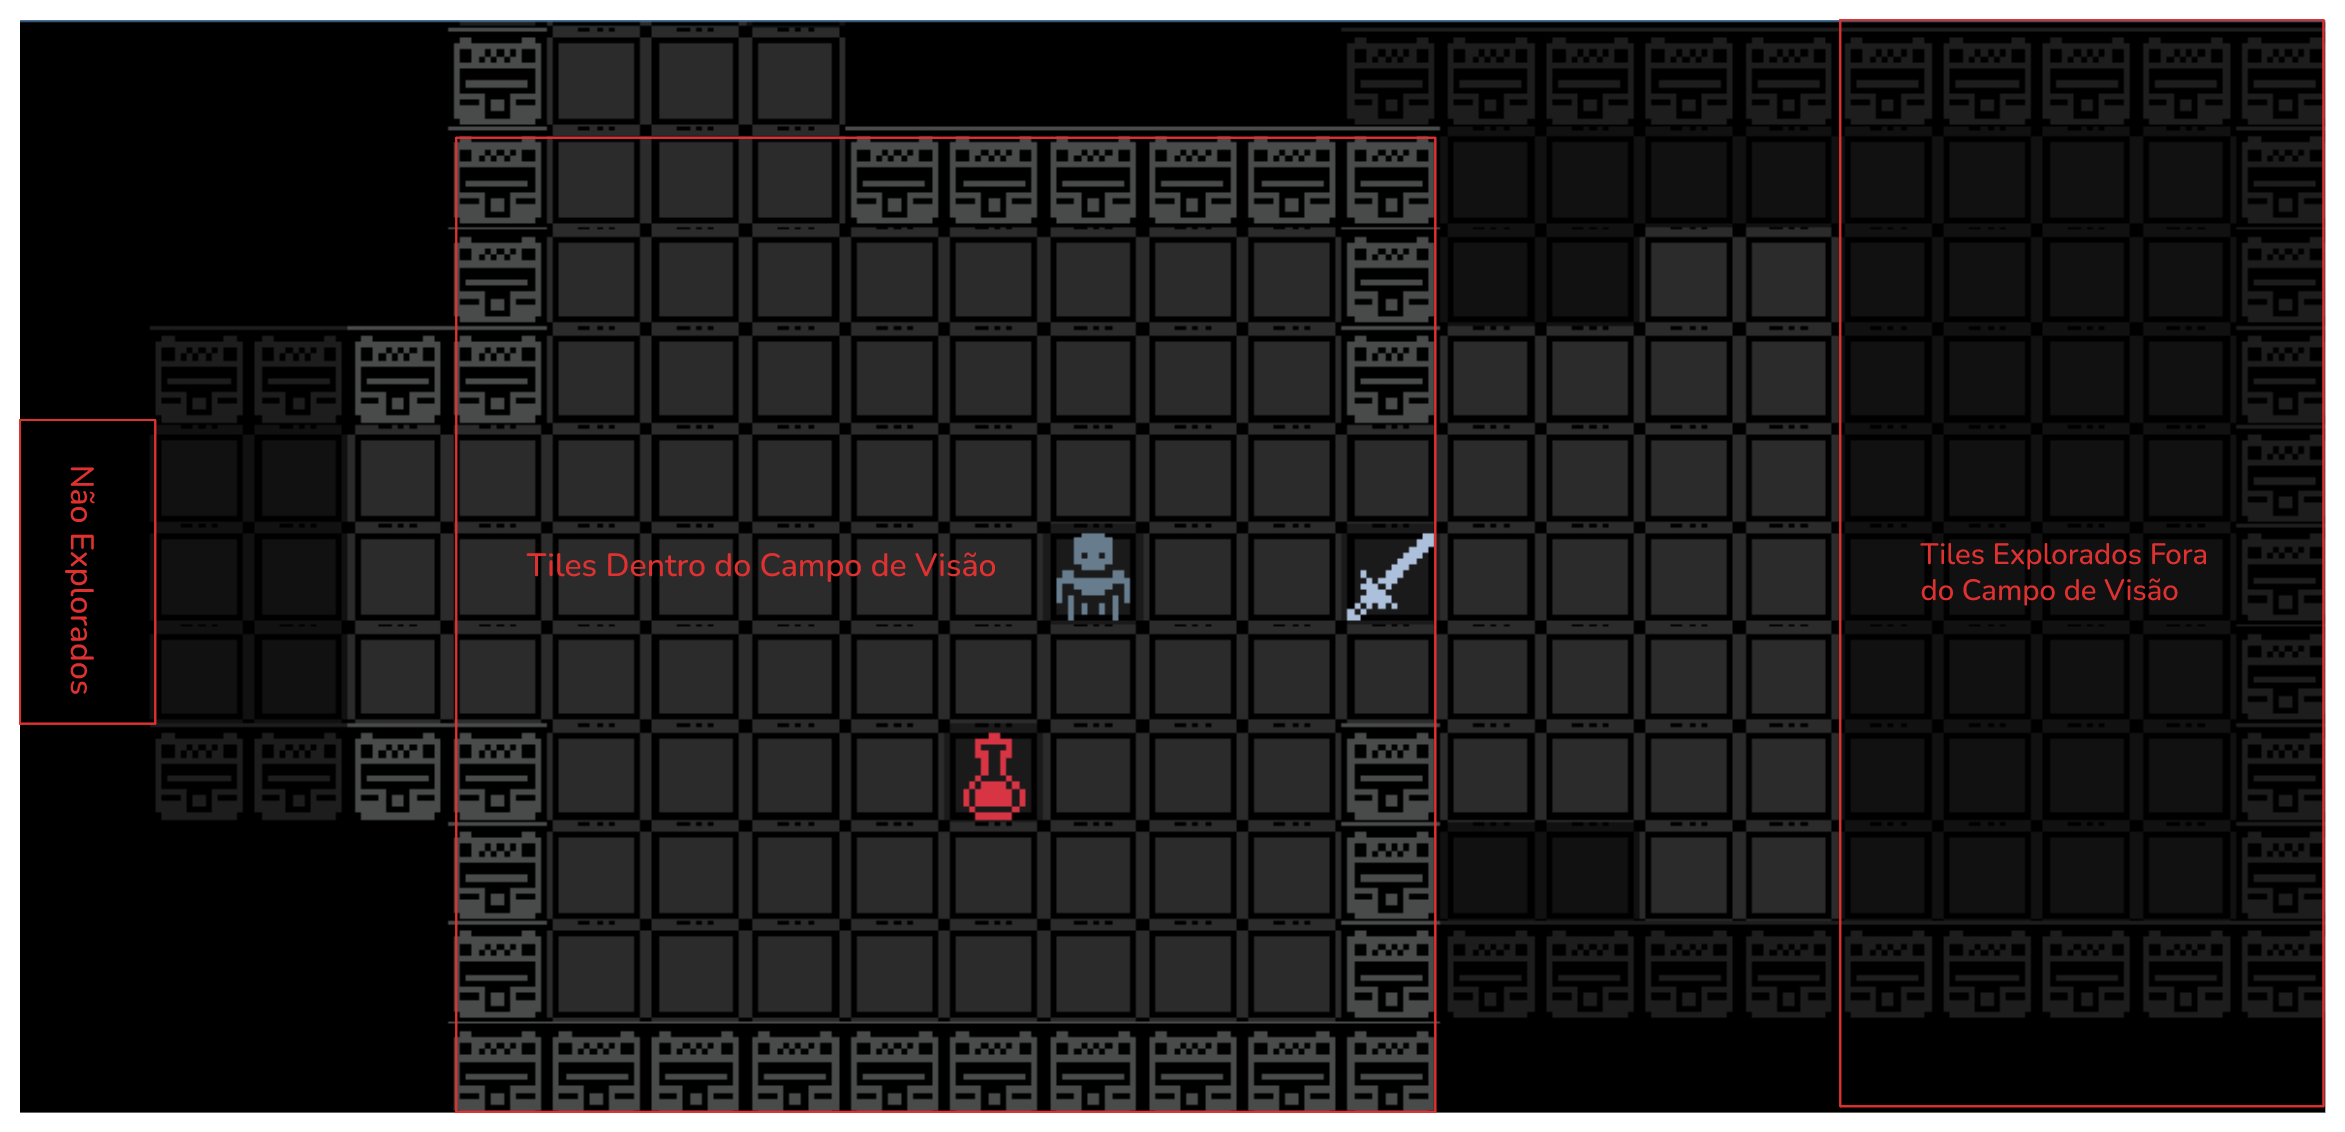
\includegraphics[width=12cm]{figuras/field_of_view.png}
    }{
        \Fonte{Elaborado pelo autor}
    }
\end{figure}

O sistema divide a renderização do mapa em três estados distintos:
\begin{enumerate}
    \item \textbf{Tiles Visíveis:} A área iluminada ao redor do jogador, onde
          entidades (inimigos e itens) são renderizadas em tempo real.
    \item \textbf{Tiles Explorados (Fora do \gls{FOV}):} Áreas que o jogador já visitou,
          mas que não estão em sua linha de visão direta no momento. Estes \textit{tiles}
          permanecem visíveis, porém escurecidos e estáticos (não mostram movimentação
          de inimigos), servindo como memória espacial para o jogador.
    \item \textbf{Tiles Não Explorados:} Áreas completamente ocultas (preto),
          que representam o desconhecido.
\end{enumerate}

Este mecanismo garante que o jogador tenha apenas uma noção parcial da estrutura
da masmorra, preservando a sensação de surpresa e perigo ao adentrar novas salas.

\subsection{Geração Procedural e Progressão de Dificuldade}

A estrutura física das masmorras é criada utilizando o
Algoritmo~\ref{alg:dungeon_gen_high_level} descrito na metodologia. A
Figura~\ref{fig:dungeons_gen} demonstra três gerações distintas de níveis da
masmorra, evidenciando a variabilidade topológica obtida.

\begin{figure}[!ht]
    \centering
    \Caption{\label{fig:dungeons_gen} Três exemplos de níveis gerados
        proceduralmente com diferentes configurações espaciais.}
    \UFCfig{}{
        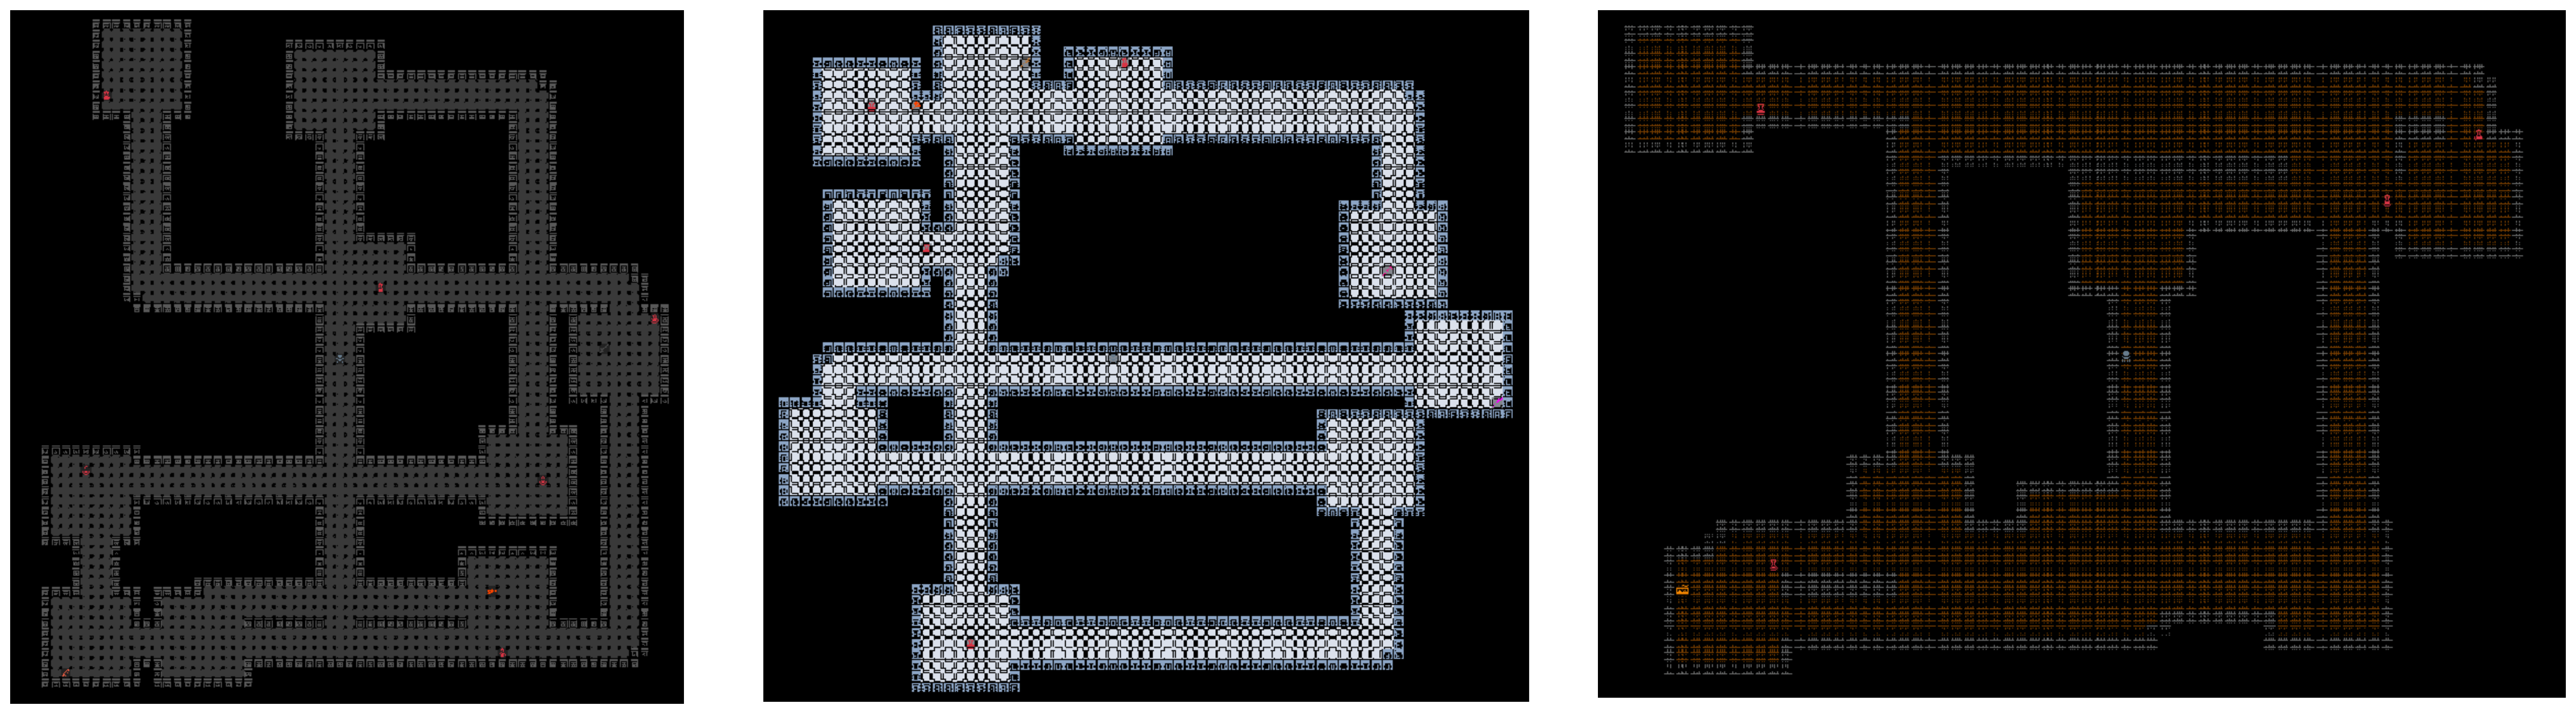
\includegraphics[width=12cm]{figuras/three_diferent_dungeons_generations.png}
    }{
        \Fonte{Elaborado pelo autor}
    }
\end{figure}

Cada mapa é composto por múltiplas salas retangulares interconectadas por
corredores. Após a definição da geometria, o sistema popula as salas com itens e
inimigos baseando-se nos metadados de \textit{rarity}, \textit{threat} e
\textit{weight} definidos pelo \gls{LLM}. O algoritmo de povoamento utiliza uma
curva de probabilidade ajustada pela profundidade do nível: itens raros e
inimigos com alto nível de ameaça possuem chances mínimas de aparecer nos
primeiros níveis, mas tornam-se progressivamente mais comuns conforme o jogador
desce para profundidades maiores. Esta abordagem assegura não apenas a
integridade estrutural do mapa, mas também um senso tangível de progressão de
dificuldade e recompensa.